\documentclass[11pt, a4paper]{article}
\usepackage[english]{babel}
\usepackage[utf8]{inputenc}
\usepackage{fancyhdr}
\usepackage{lastpage}
\usepackage{datetime}
\usepackage{indentfirst}
\usepackage{hyperref}
\usepackage{appendix}
\usepackage{amsmath}
\usepackage{amssymb}
\usepackage{amsfonts}
\usepackage{mathtools}
\usepackage{siunitx}
\usepackage{cancel}
\usepackage{tabularray}
\usepackage{multirow}
\usepackage{array}
\usepackage{hhline}
\usepackage{makecell}
\usepackage{courier}
\usepackage[font=small, skip=0pt]{caption}
\usepackage[font=scriptsize, skip=0pt]{subcaption}
\usepackage{float}
\usepackage{graphicx}
\usepackage{listings}
\usepackage{xcolor}
\usepackage{matlab-prettifier}
\usepackage[T1]{fontenc}
\usepackage{lmodern}
\usepackage{bigfoot}
\usepackage{filecontents}
\usepackage[nottoc]{tocbibind}

\graphicspath{ {./mathimages/} }

\newdateformat{Datea}{\THEDAY\ \monthname[\THEMONTH] \THEYEAR}
\newdateformat{Dateb}{\monthname[\THEMONTH] \THEYEAR}

%\allowdisplaybreaks
\DeclareMathOperator{\cosec}{cosec}
\DeclareMathOperator{\cotan}{cotan}
\DeclareMathOperator{\sech}{sech}
\DeclareMathOperator{\cosech}{cosech}
\DeclareMathOperator{\arcsec}{arcsec}
\DeclareMathOperator{\arccot}{arccot}
\DeclareMathOperator{\arccsc}{arccosec}
\DeclareMathOperator{\arccosh}{arccosh}
\DeclareMathOperator{\arcsinh}{arcsinh}
\DeclareMathOperator{\arctanh}{arctanh}
\DeclareMathOperator{\arcsech}{arcsech}
\DeclareMathOperator{\arccsch}{arccsch}
\DeclareMathOperator{\arccoth}{arccoth}
\DeclareMathOperator{\arsinh}{arsinh}
\DeclareMathOperator{\arcosh}{arcosh}
\DeclareMathOperator{\artanh}{artanh}

\DeclareMathOperator{\cis}{cis}

\pagestyle{fancy}
\fancyhf{}
\rhead{Hatam Barma}
\chead{\begin{tabular}[t]{@{}l@{}}\\Mathematics and Further Mathematics Pure Revision Summary\end{tabular}}
\lhead{\Dateb\today}
\cfoot{Page \thepage}

\renewcommand{\thesection}{\arabic{section}} 

\renewcommand{\thesubsection}{\thesection.\arabic{subsection}}

\setcounter{section}{11}

\allowdisplaybreaks

\fancypagestyle{plain}{
\fancyhf{}
\renewcommand{\headrulewidth}{0pt}}

\hypersetup{
    colorlinks,
    citecolor=black,
    filecolor=black,
    linkcolor=blue,
    urlcolor=magenta!70!black
}

\begin{document}


\begin{titlepage}
   \begin{center}
       \vspace*{2.5cm}
	\huge
       \textbf{A-Level Mathematics and Further Mathematics Pure Revision Summary} \\
	\vspace{1cm}
	\Large
       \textbf{Chapter 12: Numerical methods}
            
       \vspace{1.5cm}
	\LARGE
       \textbf{Hatam Barma} \\
	\vspace{0.75cm}
       \normalsize
       \emph{Compiled on \Datea\today} \\

       \vfill
        

	E-mail: hatam.barma@gmail.com
   \end{center}
\end{titlepage}


\tableofcontents

\clearpage
\section{Numerical methods}
\vspace{0.5cm}


\subsection{Decimal search, or numerical analysis}
\begin{itemize}
\item A Level M Year 2 \hspace{1cm} \phantom{ AS / } Pages 298 -- 302
\end{itemize} \par
In order to find the roots of an equation,  we can perform a numerical analysis of the curve, as opposed to solving it directly. This can be done by taking an interval, for example $x=1$ and $x=2$ in this example. We then compute values of the function between these limits, and find the interval at which it changes sign. We then recompute values between these new limits in order to improve the accuracy of the answer.
\begin{itemize}
\item[Note:] At the final stage, compute the value of the function half way between the final set of limits in order to determine which limit it rounds to.
\end{itemize}
\vspace{0.5cm}


\subsection{Newton-Raphson Iteration}
\begin{itemize}
\item A Level M Year 2 \hspace{1cm} \phantom{ AS / } Pages 304 -- 312
\end{itemize} \par
\begin{figure}[H]
\centering
\scalebox{.5}{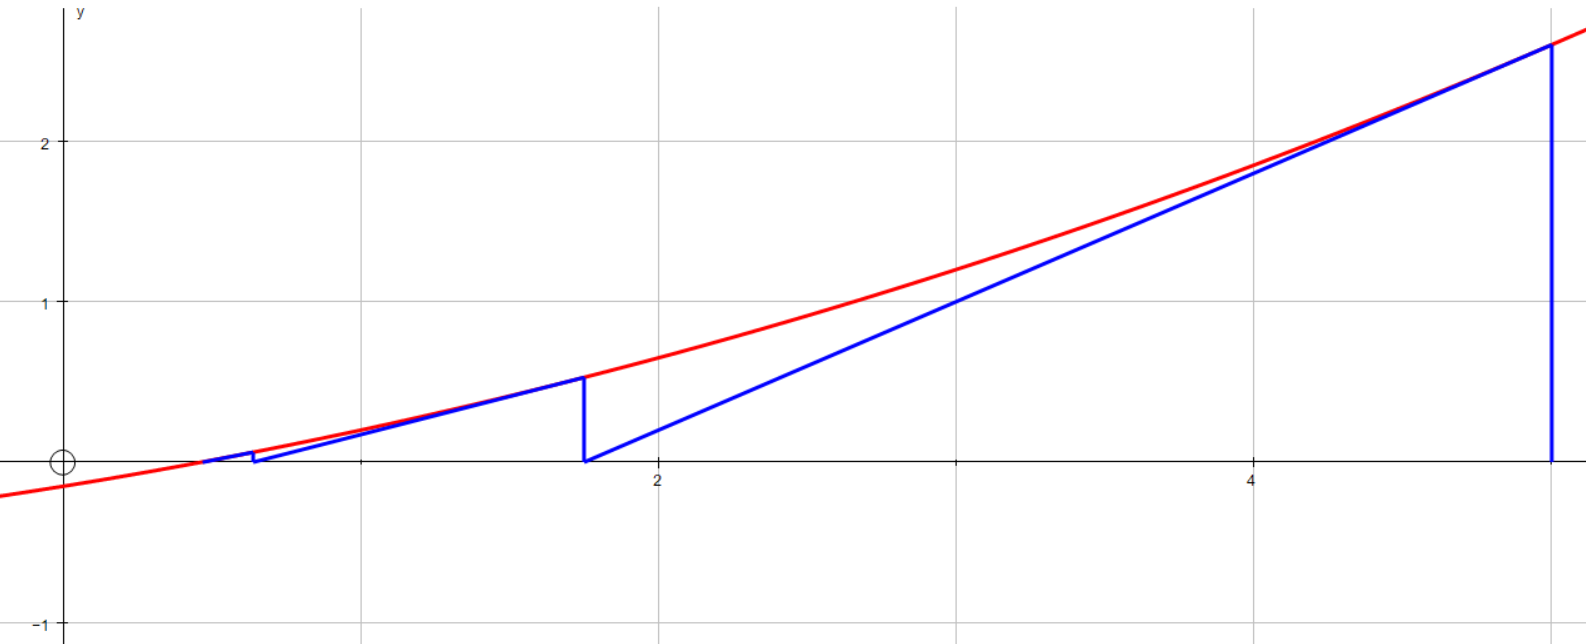
\includegraphics[width=\textwidth]{newtonraphson}}
\end{figure}
A Newton-Raphson iteration is another method for finding a root of an equation. In order to perform one, draw a tangent and follow it towards a root. At its intersection with the $x$-axis, recalculate the tangent with the new $x$-coordinate, and follow the new tangent towards the root. \newline \par

For the curve $y=f(x)$, the tangent at any given point, $\left(x_{n},f\left(x_{n}\right)\right)$ has equation
\begin{equation*}
y-f\left(x_{n}\right)=f'\left(x_{n}\right)\cdot\left(x-x_{n}\right) \\
\end{equation*}
The root of this equation is where $x=x_{n+1}$, and $y=0$. Therefore
\begin{align*}
0-f\left(x_{n}\right)&=f'\left(x_{n}\right)\cdot\left(x_{n+1}-x_{n}\right) \\
& \\
x_{n+1}&=x_{n}-\frac{f\left(x_{n}\right)}{f'\left(x_{n}\right)}
\end{align*}
\vspace{0.5cm}


\subsection{Fixed point iteration}
\begin{itemize}
\item A Level M Year 2 \hspace{1cm} \phantom{ AS / } Pages 313 -- 326
\end{itemize} \par
\begin{figure}[H]
\centering
\scalebox{.5}{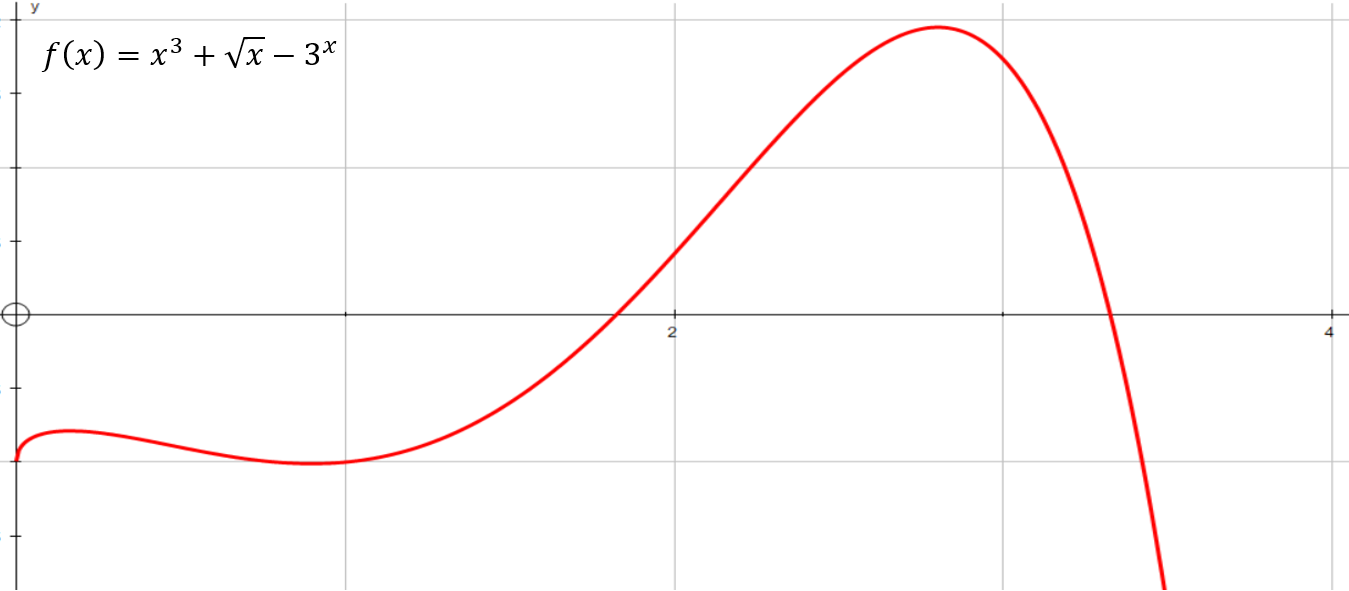
\includegraphics[width=\textwidth]{fixedpointiteration}}
\end{figure}
\begin{itemize}
\item[-] A fixed point of an iterated function is a number that an iteratively defined function converges to from various starting inputs
\item[-] A stable fixed point is one which the function converges to from various inputs. An unstable fixed point returns itself only when it itself is the input.
\end{itemize}
To find an iteration of a function to find a root, rearrange the function to give $x$ in terms of $x$. For example, take the function $x^{5}-3x^{4}+1=0$
\begin{align*}
x&=\sqrt[4]{\frac{x^{5}+1}{3}} & &\text{which converges to }x=0.82328\ldots \\
x&=\sqrt[5]{3x^{4}-1} & &\text{which converges to }x=0.85667\ldots \\
x&=\frac{x^{4}-1}{x^{4}} & &\text{which converges to }x=2.98745\ldots \\
\end{align*}
Another way of thinking about this then is thinking of the roots of $f(x)$ being at the point of the intersection between $y=g(x)$, a function which gives $x$ in terms of $x$, and $y=x$. However the iteration will only converge under the condition that $\left| g'\left( x_{root} \right) \right|<1$ \newline \par

\noindent If:
\begin{flalign*}
0\leq\,&g'\left( x_{root} \right)\leq1 & &\text{The iteration will converge stepwise} \\
1\leq\,&g'\left( x_{root} \right) & &\text{The iteration will diverge stepwise} \\
-1\leq\,&g'\left( x_{root} \right)\leq0 & &\text{The iteration will converge as a spiral} \\
&g'\left( x_{root} \right)\leq-1 & &\text{The iteration will diverge as a spiral}\\
\end{flalign*}
\vspace{0.5cm}


\end{document}